%% The first command in your LaTeX source must be the \documentclass command.
\documentclass[manuscript]{acmart}

\usepackage{listings}

%%
%% \BibTeX command to typeset BibTeX logo in the docs
\AtBeginDocument{%
  \providecommand\BibTeX{{%
    Bib\TeX}}}

%% Rights management information.  This information is sent to you
%% when you complete the rights form.  These commands have SAMPLE
%% values in them; it is your responsibility as an author to replace
%% the commands and values with those provided to you when you
%% complete the rights form.
%\setcopyright{acmcopyright}
%\copyrightyear{2018}
%\acmYear{2018}
%\acmDOI{XXXXXXX.XXXXXXX}

%% These commands are for a PROCEEDINGS abstract or paper.
%%\acmConference[Conference acronym 'XX]{Make sure to enter the correct
%%  conference title from your rights confirmation emai}{June 03--05,
%%  2018}{Woodstock, NY}
%%\acmPrice{15.00}
%%\acmISBN{978-1-4503-XXXX-X/18/06}


%%
%% For managing citations, it is recommended to use bibliography
%% files in BibTeX format.
%%
%% You can then either use BibTeX with the ACM-Reference-Format style,
%% or BibLaTeX with the acmnumeric or acmauthoryear sytles, that include
%% support for advanced citation of software artefact from the
%% biblatex-software package, also separately available on CTAN.
%%
%% Look at the sample-*-biblatex.tex files for templates showcasing
%% the biblatex styles.
%%

%%
%% The majority of ACM publications use numbered citations and
%% references.  The command \citestyle{authoryear} switches to the
%% "author year" style.
%%
%% If you are preparing content for an event
%% sponsored by ACM SIGGRAPH, you must use the "author year" style of
%% citations and references.
%% Uncommenting
%% the next command will enable that style.
%%\citestyle{acmauthoryear}


%%
%% end of the preamble, start of the body of the document source.
\begin{document}

\title{Integrating OSLO semantics in word processors}

%%
%% The "author" command and its associated commands are used to define
%% the authors and their affiliations.
%% Of note is the shared affiliation of the first two authors, and the
%% "authornote" and "authornotemark" commands
%% used to denote shared contribution to the research.
%\author{Dwight Van Lancker}
%\authornote{Both authors contributed equally to this research.}
%\email{dwight.vanlancker@ugent.be}
%\affiliation{%
%  \institution{IDLab, Dep. of Electronics and Information Systems, Ghent %University - imec}
%  \country{Belgium}
%}
%\orcid{1234-5678-9012}
%\author{Niels Van Durme}
%\email{niels.vandurme@ugent.be}
%\author{Eveline Vlassenroot}
%\email{eveline.vlassenroot@ugent.be}
%\affiliation{%
%  \institution{MICT, Dep. of Communication Sciences, Ghent University - imec}
%  \country{Belgium}
%}

%\author{Raf Buyle}
%\email{raf.buyle@ugent.be}
%\affiliation{%
%  \institution{IDLab, Dep. of Electronics and Information Systems, Ghent University - imec}
%  \country{Belgium}
%}
  
%\author{Peter Mechant}
%\email{peter.mechant@ugent.be}
%\affiliation{%
%  \institution{MICT, Dep. of Communication Sciences, Ghent University - imec}
%  \country{Belgium}
%}
%
%\author{Pieter Colpaert}
%\email{pieter.colpaert@ugent.be}
%\affiliation{%
%  \institution{IDLab, Dep. of Electronics and Information Systems, Ghent University - imec}
%  \country{Belgium}
%}
%  
%\author{Erik Mannens}
%\email{erik.mannens@ugent.be}
%\affiliation{%
%  \institution{IDLab, Dep. of Electronics and Information Systems, Ghent University - imec}
%  \country{Belgium}
%}


%%
%% By default, the full list of authors will be used in the page
%% headers. Often, this list is too long, and will overlap
%% other information printed in the page headers. This command allows
%% the author to define a more concise list
%% of authors' names for this purpose.
\renewcommand{\shortauthors}{Dwight Van Lancker et al.}

%%
%% The abstract is a short summary of the work to be presented in the
%% article.
\begin{abstract}
Documents issued by the government such as public tenders or policy documents often lack consistent semantics, which leads to ambiguities and misinterpretations. 
Take for example granting subsidies to companies. 
The conditions for entitlement to a subsidy are checked against the government’s authentic data sources. 
However, the various governments and administrations have different definitions of, for instance, a small and medium-sized enterprise (SME), which can be derived from a European legal framework or a financial perspective. 
The absence of uniform definitions for these terms results in a lot of duplicate efforts for both the government and the entrepreneur. 
To tackle the problem of semantics, Flanders founded an interoperability program, Open Standards for Linked Organizations (OSLO) whose primary goal is to ensure that systems exchanging data can use a common vocabulary. 
However, despite the results made by OSLO, they do not reach policy-makers working mainly on the legal and organizational levels. 
We developed two tools to close this gap and make semantic agreements available at these levels. 
With OSLO Lookup, we provide a simple user interface that lets users query the semantics assets, while the OSLO365 plugin allows embedding the semantic assets in a Microsoft Word document. 
To assess the relevance and usability of these tools, servants of a local administration were interviewed. 
This paper outlines that semantic agreements that are mainly used on the data level can provide added value at an organizational and legal level as well.
\end{abstract}

%% TODO
\ccsdesc[500]{General and reference~Computing standards}
\ccsdesc[300]{Applied computing~E-government}
\ccsdesc[300]{Information systems~Resource Description Framework (RDF)}

%%
%% Keywords. The author(s) should pick words that accurately describe
%% the work being presented. Separate the keywords with commas.
\keywords{Interoperability, Linked Data, e-Government, Semantic Web, Word processors}
%% A "teaser" image appears between the author and affiliation
%% information and the body of the document, and typically spans the
%% page.


%%
%% This command processes the author and affiliation and title
%% information and builds the first part of the formatted document.
\maketitle

\section{Introduction}
In 2015, the founder of the World Economic Forum, Klaus Schwab, announced that the world was undergoing its fourth industrial revolution. 
He defines the Fourth Industrial Revolution as ``a world in which virtual and physical systems of manufacturing cooperate with each other in a flexible way at the global level''\cite{schwab2017fourth}. 
One of the pillars of this revolution is \emph{data}, which is used at various levels, e.g. systems use data to communicate to each other, but also at the political level as policy-makers use data-based tools to justify their decisions.
In the past few years, governments have had to invest enormously to keep up with digitization.
In Flanders, they did this by launching a five-year plan, called "Vlaanderen Radicaal Digitaal" (VRD), which runs until 2024.
An already great result of the VRD program is called \textit{Mijn Burgerprofiel}, a smart digital assistant, which aims to provide access to multiple public services through a single entry point~\cite{buyle2018semantics}.
The ultimate goal of the VRD initiative is for the Flemish government to shift towards a digital and information-driven government.


As data has become a key pillar in the European digital economy, Europe has come up with a strategy to unlock the full potential of data, which should lead to the rise of European data spaces.
Europe defines a data space as a ``decentralized infrastructure for trustworthy data sharing and exchange in data ecosystems based on commonly agreed principles''.
In their strategy, they released a first set of guidelines, collectively called the \emph{Data Governance Act}, which aim to facilitate data sharing across member states and between different sectors \cite{designDataSpaces, dataGovernanceAct}.
An essential aspect of this architecture is \emph{interoperability} because this will be necessary for an efficient and sustainable exchange of data.
Figure \ref{architectureDataSpace} shows the building blocks that are part of a European Data Space, with a \emph{Vocabulary Provider} building block in the top-right corner, whose task it is to provide data standards, so that data can flow between the various components in the data space.

\begin{figure}[h]
  \centering
  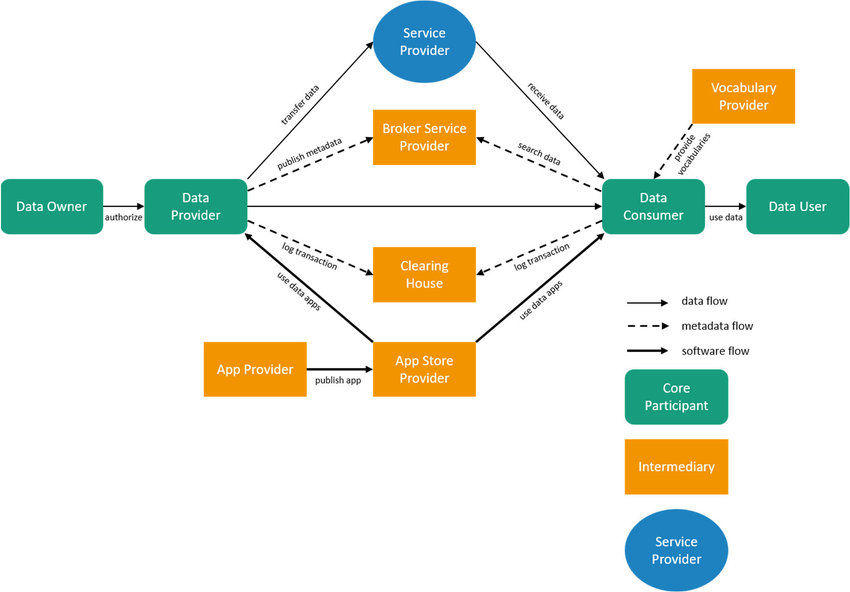
\includegraphics[width=\linewidth]{images/data-space}
  \caption{Overview of the architecture of a European Data Space\protect\footnotemark}
  \label{architectureDataSpace}
\end{figure}

\footnotetext[1]{\url{https://github.com/International-Data-Spaces-Association/idsa}}

In Flanders, the question of Vocabulary Provider is already answered with the Flemish Interoperability program, called Open Standards for Linked Organizations (OSLO). 
OSLO was aligned with the European Interoperability Framework~\footnote{\url{https://ec.europa.eu/isa2/sites/default/files/eif_brochure_final.pdf}} (EIF), which acts as a set of guidelines focused on the interoperability of digital public services.
%% TODO: add LBLOD example (Eveline)
This framework introduces four layers of interoperability: legal, organizational, semantic and technical.
The legal layer refers to aligned legislation between different organizations and policy areas. 
The second layer, organizational, refers to aligned business processes between different public administrations. 
The semantic interoperability layers refers to the definition of data content. 
For example, when two information systems are semantically interoperable, the meaning of the exchanged data is preserved and understood between the systems. 
The last layer, technical interoperability, aims at the different protocols, formats and interfaces to exchange data~\cite{eif}.
The main focus of OSLO is on the latter two interoperability layers.
Take the smart digital assistant example from above, by using OSLO, semantic and technical interoperability was ensured, making it possible to easily integrate the information systems from different administrations~\cite{buyle2018semantics}.

However, by focusing on the semantic and technical layers, the semantic agreements made by OSLO are locked on the data level, although they can provide added value at other levels as well.
This resulted in the following research question: ``\textbf{How can we support certain target groups, e.g policy-makers, at the organizational and legal level with agreements made at the semantic level?}''.

In this paper, we aim to close this gap by making semantic assets generated by OSLO, available to target audiences at the organizational and legal layers by two tools.

\section{Background}

At the time of writing, Flanders has 300 local governments which provide over 800 different products and services, often using applications from various software vendors. 
Data coming from those different systems often have a different data model, are in a different format, and do not necessarily have the same semantics. 
This results in the creation of vertical data silos and makes it challenging to exchange high-quality data. 
To resolve these interoperability problems, in 2012, an interoperability initiative was founded, called \textit{Open Standards for Linked Organizations} (OSLO)~\cite{buyle2016oslo}.
Since then, OSLO has facilitated the co-creation of data standards in more than 100 domains, capturing over 4000 definitions. 
The realization of data standards in Flanders is done by following a well-defined process and methodology, called ``OSLO Process \& Method'' \footnote{\url{https://data.vlaanderen.be/cms/Proces_en_methode_voor_de_erkenning_van_datastandaarden_v1.0.pdf}}.
The OSLO process is aligned with international best practices of ISA, W3C, and OpenStand, ensuring qualitative data standards and a governance structure.
Through various workshops together with domain experts, a domain model is established as a UML (Unified Modelling Language) class diagram. 
Using UML to create the data model, a view is provided of which relations exist between various objects in the domain, and how data should be exchanged in general.
Based on this UML data model, a vocabulary is generated in both a human and machine-readable format, by re-using the principles of Linked Data~\footnote{\url{https://www.w3.org/DesignIssues/LinkedData.html}}.

Linked Data is defined as a set of design principles to share machine-readable information on the Web, as defined by the founder of the World Wide Web, Tim Berners-Lee in 2006. 
The first design principle is about identifying things and states that unique resource identifiers (URIs) should be used as names for things. 
The second principle expands the first by stating that HTTP URIs should be used, so that users can look up those names. 
The third principle is about information coupled to the HTTP URIs. 
When a user enters an HTTP URI in their browser, they should get useful information in return. 
That information should be described by using a standardized format, called the Resource Description Framework (RDF). 
RDF is a directed graph that contains statements. 
These RDF statements consist of three parts, a subject, a predicate, and an object, and are therefore also called \textit{triples}. 
For example: ``John knows Jane'', where John is the subject, ``knows'' the predicate, and Jane the object. 
Each part in the triple is represented by a URI, whereas the object can also be a literal value (e.g. string, integer, …). 
The last design principle is about linking to other data by including HTTP URIs to other entities in your data, allowing users to discover more information on the Web.

All properties and classes on an OSLO UML data model are assigned URIs, uniformly identifying each term within the domain model.
These URIs are not assigned at random, but by aligning with already existing data standards. 
For example, the term representing a person was assigned the URI \url{http://www.w3.org/ns/person#Person}, re-using the URI and definition the term ``person'' was assigned by W3C.
In some cases, no URI exists to assign to the term, as their definition differs too much, and in that case, a new URI is created.
For example, in Flanders, to exchange data about a person, there is a mandatory property that contains the full name of a person.
However, in international standards, this does not exist, and therefore a new URI was created: \url{https://data.vlaanderen.be/ns/persoon#volledigeNaam}.

\section{Architecture}

OSLO targets the semantic and technical level, meaning the semantic agreements are mainly used to add context to data. Take for example the following code sample:
%% TODO: they should appear side by side
\noindent
\begin{lstlisting}[caption=JSON data snippet,frame=tlrb, label={lst:json}]{Name}
{
   "place": "Brussels"
}
\end{lstlisting}\hfill
\begin{lstlisting}[caption=JSON-LD data snippet,frame=tlrb, label={lst:jsonld}]{Name}
{
   "@context" : {
      "place": "https://schema.org/location"
   },
   "place": "Brussels"
}
\end{lstlisting}

Listing \ref{lst:json} shows a JSON object containing a property ``place'' with value ``Brussels''.
However, one could argue about the definition of the property ``place''.
This problem is solved by listing \ref{lst:jsonld}. 
This code snippet is a Linked Data serialization, called JSON-LD, and adds semantics to the data by assigning URIs, with ``place'' being assigned the URI ``https://schema.org/location'' in this example. 
Users can enter that URI in their browser to discover which definition is attached to this URI and by extension the property ``place''.

As Linked Data is the solution to add semantics to data and resolve ambiguities and misinterpretations, it is only used at the data level.
People at the legal and organizational levels almost never come in contact with these semantic agreements, although they can provide added value to legal documents for example.

\subsection{OSLO Lookup}

%% TODO: change deploy URL of OSLO Lookup
%% TODO: insert link to GitHub page with README instructions on how to use it
In order to make the semantic agreements available to target groups at the organizational and legal level, we created a simple user interface, called \textit{OSLO Lookup}, which allows users to enter multiple keywords and check if they were defined within OSLO.
The code of OSLO Lookup is publicly available on GitHub~\footnote{\url{https://github.com/informatievlaanderen/OSLO-Lookup}}.

Although this is an excellent first step toward semantic agreements being used at the organizational and legal levels, constantly using the OSLO Lookup functionality to check if a word exists in OSLO can be pretty cumbersome.
Therefore, we looked for a way in which we could make the semantic agreements available within the work environment. This was achieved by developing an add-in for Microsoft Word, called \textit{OSLO365}, enabling users to embed semantics in their Word documents.

\begin{figure}[h]
  \centering
  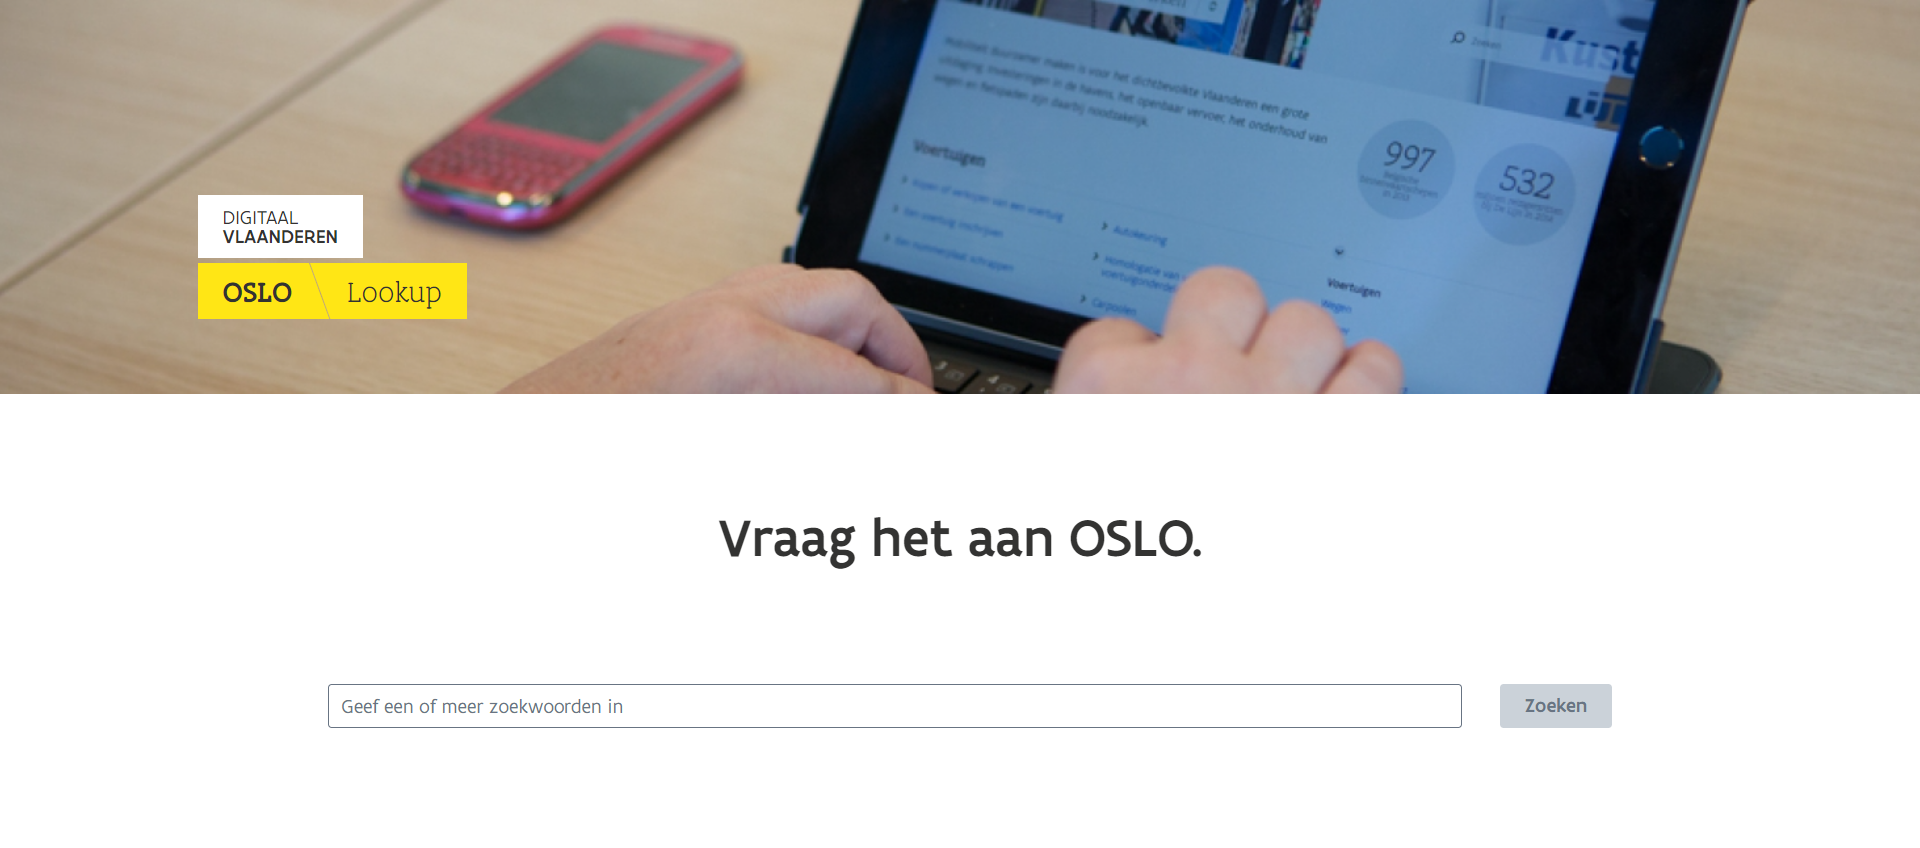
\includegraphics[width=\linewidth]{images/oslo-lookup}
  \caption{With OSLO Lookup, users can enter multiple keywords to check if they are defined in OSLO.}
  \label{osloLookup}
\end{figure}

\subsection{OSLO Lookup integrated in OSLO365}

The Office Word add-in has multiple functions to assist the user in adding semantics to their document. 
Firstly, we integrated the OSLO Lookup functionality in the add-in, allowing users to enter a keyword in a search field and relevant results will be shown to the user, as shown on figure \ref{oslo-add-in-1}. 
To make it even more user-friendly, users can also select a word in the document and the add-in will automatically look up the selected word. 
To actually add semantics to their documents, users can add the definition of a word along with their URI as a foot or endnote to the document, as shown in figure \ref{oslo-add-in-2}.
By embedding the URI and its definition in the document, other readers or contributors do not have to deal with ambiguities anymore.

\begin{figure}
\centering
\begin{minipage}{.5\textwidth}
  \centering
  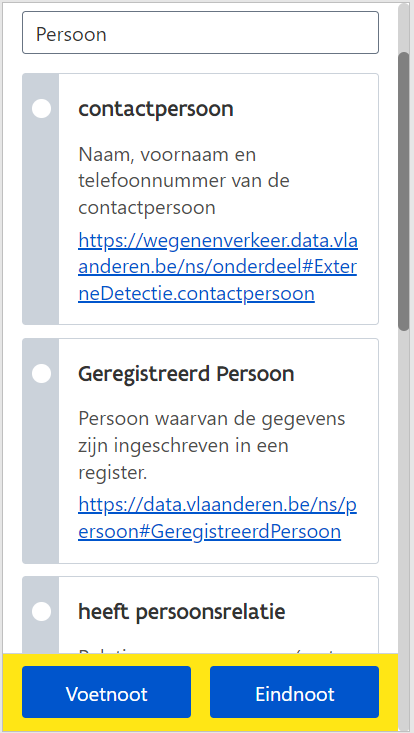
\includegraphics[scale=.5]{images/oslo-add-in-1}
  \caption{The OSLO add-in shows all the results for a keyword or a selected word in the document. In this example, results are shown for the keyword ``Persoon'' (Person in English)}
  \label{oslo-add-in-1}
\end{minipage}%
\begin{minipage}{.5\textwidth}
  \centering
  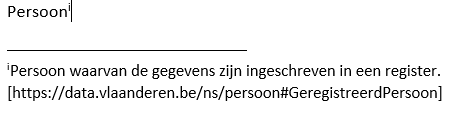
\includegraphics[scale=.5]{images/oslo-add-in-2}
  \caption{The OSLO add-in allows to embed an OSLO definition in the Word document as a foot or endnote. In this example, a definition for the word ``persoon'' is embedded as an endnote in the document, alongs with its URI.}
  \label{oslo-add-in-2}
\end{minipage}
\end{figure}

This functionality above is a great first way to add semantics to Word documents but can be time-consuming for large documents. 
Therefore, the add-in also has a function to scan the whole document. 
When done scanning, the add-in will guide the user through his Word document and indicate for which words it has results. 
The user can individually decide for each word what definition to insert into the document. 
The last functionality of this add-in is a dictionary. 
As a user, you want to easily find a commonly used definition. 
Therefore, users can add definitions to their dictionary making it immediately available if they click on the dictionary. Figure \ref{oslo-dictionary-2} shows that users can access their dictionary to check which definitions are saved, insert them as a foot or endnote or remove them if necessary.
On top of this, if a user searches a word or lets the add-in scan the document, definitions added to the user's dictionary will be marked in yellow and shown as the first result, as shown in figure \ref{oslo-dictionary-1}. The code of the OSLO365 plugin is publicly available on GitHub~\footnote{\url{https://github.com/informatievlaanderen/OSLO365-plugin}}.

\begin{figure}
\centering
\begin{minipage}{.5\textwidth}
  \centering
  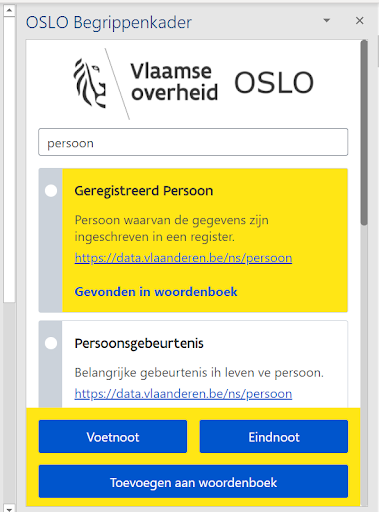
\includegraphics[scale=.5]{images/oslo-dictionary-1}
  \caption{Definitions saved in the dicionary are marked in yellow when they appear in the search results}
  \label{oslo-dictionary-1}
\end{minipage}%
\begin{minipage}{.45\textwidth}
  \centering
  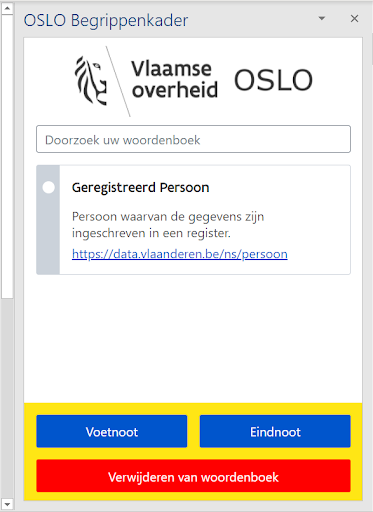
\includegraphics[scale=.5]{images/oslo-dictionary-2}
  \caption{Users can consult their dictionary and remove a definition from their dictionary}
  \label{oslo-dictionary-2}
\end{minipage}
\end{figure}

\section{Relevance and usability assessment}

To assess the relevance and usability of the developed OSLO365 add-in, we took an explorative ethnographic research approach. 
This approach involved interviewing multiple local servants at an administration of a local mid-sized municipality in Flanders. 
Using a semi-structured interview guide, we talked to six public servants from different departments with distinct roles and responsibilities, asking them to perform their daily tasks and to define specific terms or concepts using the Office add-in. 
The ``think aloud'' protocol~\cite{jaaskelainen2010think} enabled us to identify information that is concentrated on during problem-solving as well as information used to facilitate problem resolution. 
When asked to define a particular concept (e.g., `Gemeente' [Municipality]), most respondents interacted with the thesaurus function - expecting a full dictionary containing all OSLO vocabulary terms - rather than the therefore intended search function. 
The thesaurus function was generally well-received, with most civil servants finding it helpful in defining frequently used terms or concepts. 
The search functionality was also met with positive feedback, with respondents stating that it felt natural and intuitive to use.  
The functionality `document scan' was the most criticized affordance; after scanning a document, the add-in would only allow public servants to navigate through a list of matched terms by clicking the buttons `previous' or `next', with one public servant stating: ``I am flabbergasted that such a useful feature as the document scan is implemented in such a non-efficient way.''. 
The functionality however also received praise as it was identified as a useful feature to make people aware of how ambiguous and unclear their day-to-day jargon could be for others outside of their domain.  
In general, respondents told us that usability is key and that the add-in should be supported in the whole administration of the municipality for them to use it individually in their daily tasks. 
The add-in proved to be relatively easy to use, as no respondent had any particular issues when working with it. 

\section{Discussion and future work}

To increase interoperability, Flanders has invested intensely in the OSLO program, with OSLO targeting the semantic and technical interoperability layer, which provides a great added value at the data level. 
However, for target audiences at the organizational and legal level, there is a barrier to use these semantic agreements, as they rarely come into contact with the actual data level.
This results in the fact that the efforts made by OSLO often stay at the semantic and technical interoperability layers, although they can provide an added value at the other layers as well.

In this paper, we introduced two tools in order to smooth the flow of semantic agreements to the legal and organizational level. 
With OSLO Lookup, we show that we can easily provide an application to  unlock the semantic agreements at the data level and make them available at other levels as well.
With the Office add-in, OSLO365, we make the semantic agreements available for Microsoft Word users, who can look up semantic agreements and incorporate them in their Word documents. 
Doing this will decrease the number of ambiguities or misinterpretations by readers of these documents. 
The interviews with the public servants of a local administration demonstrate that these tools allow semantic assets to be used at the organizational and legal levels, and therefore answers our research question. 
The interviewees also mentioned that in order to move away from their known and trusted working patterns, it is essential for them to be made aware of the benefits that such a move could provide for them. 
This will be a key working point for OSLO in the future.

%% TODO: insert links to GitHub
As OSLO is a Flemish initiative and all semantic assets have their definitions written in Dutch, which makes both OSLO Lookup and the Word add-in only usable in a Dutch context. 
Nevertheless, the code of these tools is publicly available on GitHub, so that it can be a source of inspiration for initiatives in other languages.

In addition to assigning URIs to terms in a UML data model, OSLO also uses URIs to uniquely identify data objects. 
For example, each address in Flanders has a unique HTTP URI. Using the Linked Data principles, entering this HTTP URI in the browser, useful information about the address will be returned. 
The useful information can be both human and machine-readable and is compliant with the OSLO data model for addresses. 
In the future, we will be doing research on how we can evolve to evidence-based documents by also making these data URIs available for the tools. 
For example, if someone enters an address in their document, the add-in should be able to retrieve the HTTP URI of that address and add it to the document.
What remains to be developed then, is the organizational aspect of implementing such a tool within a public administration.

\section{Acknowledgments}

This work was partially supported by KNoWS (IDLab - Ghent University), Proximus, Microsoft, and Digitaal Vlaanderen.

\bibliographystyle{ACM-Reference-Format}
\bibliography{references}

\end{document}
\endinput
%%
%% End of file `sample-acmsmall-conf.tex'.
